
\documentclass[journal]{IEEEtran}

\usepackage{xcolor,soul,framed} %,caption
\colorlet{shadecolor}{yellow}
\usepackage[pdftex]{graphicx}
\graphicspath{{../pdf/}{../jpeg/}}
\DeclareGraphicsExtensions{.pdf,.jpeg,.png}
\usepackage[cmex10]{amsmath}
\usepackage[all]{nowidow}
\usepackage{array}
\usepackage{mdwmath}
\usepackage{mdwtab}
\usepackage{threeparttable}
\usepackage{amsmath}
\usepackage{cite}
\usepackage{graphicx}
\usepackage[all]{nowidow}
\usepackage{eqparbox}
\usepackage{url}
\usepackage{todonotes} % added
\usepackage{xcolor}
\usepackage{dblfloatfix}
\usepackage{multirow}

\usepackage{subfigure}
\hyphenation{op-tical net-works semi-conduc-tor}
\clubpenalty=9996
\widowpenalty=9999
\brokenpenalty=4991
\predisplaypenalty=10000
\postdisplaypenalty=1549
\displaywidowpenalty=1602

%% added
\newcommand{\RomanNumeralCaps}[1]
    {\MakeUppercase{\romannumeral #1}}


%=== TITLE & AUTHORS ====================================================================
\begin{document}
%\bstctlcite{IEEEexample:BSTcontrol}
 %   \title{Design and Effect of Common DC-Bus Parallel Connected Inductive Power Transfer Systems}
%  \author{Hakan~Polat,
%      Enes~Ayaz,
%      Og\"{u}n Altun,
%      Ozan~Keysan
%}  

\title{ Fault Tolerant Multi-Tx/Multi-Rx Inductive Power Transfer System with a Resonator Coil}
        \author{Enes~Ayaz, Og\"{u}n Altun, Hakan~Polat, and Ozan~Keysan
% <-this % stops a space
			 \thanks{ Enes~Ayaz, Og\"{u}n Altun,  H. Polat and Ozan~Keysan are with Middle East Technical University, Department of Electrical and Electronics Engineering, Ankara, Turkey. Email: keysan@metu.edu.tr 
}% <-this % stops a space
\thanks{Corresponding Author: Ozan Keysan, keysan@metu.edu.tr
}% <-this % stops a space
}
\maketitle
\begin{abstract}
This paper presents a novel multi-transmitter (Tx) / multi-receiver (Rx) inductive power transfer system. 
Compared to conventional single-Tx/single-Rx systems, multi-Tx/multi-Rx topologies increase reliability and fault tolerance. 
However, unequal power distribution is challenging in these systems due to coupling differences, which prevents them from operating at rated power or requires over-designed modules.
This study proposes the addition of a middle-stage resonator (MSR) that balances power distribution by separating direct couplings between Tx and Rx coils. Thus, it increases reliability and fault tolerance.
Direct couplings between Tx and Rx coils are avoided via the proposed coil structure, which also provides rotational symmetry.
Moreover, an analytical method is proposed to avoid bifurcation, which reduces switching losses.
Then, the fault tolerance analysis on multi-Tx/multi-Rx systems and optimum selection of module numbers are investigated. 
Finally, a 1kW 2Tx/1MSR/4Rx prototype is established to continue operation under single-Tx, single-Rx, and double-Rx open circuit faults.


\end{abstract}
\begin{IEEEkeywords}
Wireless power transfer, inductive power transfer, modular design, resonator coil,  common DC bus, fault tolerance, reliability
\end{IEEEkeywords}

\IEEEpeerreviewmaketitle
\vspace*{-5mm}
\section{Introduction} 
%%%%%%%% 
Inductive power transfer (IPT) systems became prevalent in numerous applications~\cite{heart_IPT,roadway,EV,battery,consumer}. 
They provide cordless, space-free, and reliable solutions to transfer power using the loosely magnetically coupled single-transmitter (single-Tx) and single-receiver (single-Rx) coils~\cite{free-positioning,robust}. 
Thanks to their advantages, such as increased transmission distance~\cite{increased_tr_dis}, high misalignment tolerance~\cite{misalinged_multicoil,misalignment_3coil}, and fault tolerance~\cite{fault_tolerant} compared to single-Tx/single-Rx IPT systems,
multi-Tx/multi-Rx systems have recently gained popularity in dynamic applications such as EV chargers, unmanned aerial vehicles, and consumer/industrial electronics~\cite{EV_dynamic,UAV,industrial}.
Coupling coefficients and Tx/Rx inductances are time-varying in these dynamic applications~\cite{variable_coupling}, resulting in a change in the resonant frequency, power, and efficiency, which in turn result in reliability and fault issues.

%%%%%%%%%%%%%%
Multi-Tx/multi-Rx systems provide flexible mobility, and they can supply rated
power with higher efficiencies even if transmitters and receivers are misaligned~\cite{dynamic_flex,interoperable,uniform}.
They create modular structures, and the system can transfer rated power under faulty conditions.
Besides, the power ratings of these IPT systems can be increased just by increasing the number of Tx/Rx coils, and the current and voltage ratings can be adjusted via the number of series/parallel connections of modules~\cite{scalable,extendpower,SP-power}. 
%%%%%%%%%%%%

Multi-Tx/multi-Rx systems have power-sharing issues due to coupling differences coming from the nature of dynamic applications, which causes early aging modules and reliability problems \cite{current-sharing1,current-sharing2}. 
The conventional solution is to over-design the system. Otherwise, unequal power distribution can exceed the voltage/current ratings of the modules.
%%%%%%%%%
%%%%%%%%%%
Alternatively, an active full-bridge converter can be used on the receiver side instead of the diode rectifier to equalize the power distribution, increasing cost and complexity.
Moreover, based on the electrical connections of multiple modules, the compensation methods also affect the power distribution \cite{current-sharingComp}.
Therefore, choosing a reasonable compensation method can improve power-sharing, but this may distort other factors, such as coupling factors, resonant frequencies, etc.
%%%%%%
Another issue is to design bifurcation-free multi-Tx/multi-Rx systems.
The bifurcation phenomenon may arise in doubly compensated systems in relation to the coupling and load conditions, yielding more than one zero phase angle (ZPA) and distorting zero voltage switching (ZVS) above the resonant frequency~\cite{bifurcation}. 
Since ZVS helps to reduce the switching losses, a bifurcation-free design is preferred for higher efficiency. 
Compared to single-Tx/single-Rx systems, a bifurcation-free multi-Tx/multi-Rx system design is complex compared to single-Tx/single-Rx systems.
Although systematic design guidelines have been presented for single-Tx/single-Rx \cite{Aditya2019}, a general systematic design for multi-coil systems is not studied in the literature.
\begin{figure*}[ht!]
\centering
	\includegraphics[width=0.95\linewidth]{2p4s_with_resonator_3.pdf}
	\caption{The proposed multi-Tx/multi-Rx system with a middle-stage-resonator (MSR). a) Representation of the proposed system. b) Circuit diagram of the proposed system.}
	\label{fig:system}
\end{figure*}
This paper introduces a multi-Tx/multi-Rx IPT system for dynamic applications where either the Tx or Rx side is moving, and therefore the coupling is time-varying. Electric vehicle (EV) charging systems, radar systems, and wound-rotor synchronous machines are examples of such dynamic systems. In these applications, due to the varying coupling, maintaining power-sharing is an issue.
In this study, in order to solve this power-sharing issue, a middle-stage-resonator (MSR) coil is proposed, which is cost-efficient and simplifies operation under fault. 
Also, an analytical design methodology is proposed to avoid the bifurcation phenomenon, increasing transfer efficiency.
The main contributions of this paper can be listed as follows:
\vspace*{-1mm}
\begin{itemize}
    \item A fault-tolerant multi-Tx/multi-Rx system is proposed for dynamic applications.
    \item A systematic design procedure is presented to avoid bifurcation under dynamic conditions.
    \item Current sharing between modules is improved by introducing an MSR coil, and the current sharing is modeled for a common DC-Bus of parallel-connected Rx modules.
    \item A coil design is presented in order to minimize cross-couplings and keep the rotational symmetry.
    %  \item \hl{A fault-tolerant 1kW dynamic multi-Tx multi-Rx IPT system is experimentally verified.}
\end{itemize}

\section{System Structure and Problem Definition}
The prototype in this paper is designed as a contactless energy transfer system to replace conventional slip rings for large synchronous generators' (SG) field excitation. 
Conventional slip rings require regular maintenance, reduce reliability
especially for the applications where maintenance is difficult, such as field excitation of offshore wind turbines generators. Although a single-Tx/single-Rx IPT system can be used to eliminate mechanical problems of the conventional slip rings, the systems reliability is still questionable.
In order to solve these problems, a multi-Tx/single-MSR/multi-Rx IPT system is proposed, as shown in  Fig.~\ref{fig:system}.a.
Tx modules, MSR, and Rx modules are placed around the rotating shaft. 
The Rx modules and MSR rotate with the shaft while the Tx modules are on the stationary frame. 
Therefore, Rx and MSR coils are relatively stationary, which means their magnetic couplings are constant during rotation. 
However, magnetic couplings between Tx and the resonator coils change with rotation. 
%%%%%
The Tx side consists of full-bridge converter modules. 
The Rx side is uncontrolled and contains passive full-bridge diode rectifiers to reduce the complexity.
Rx modules are connected in parallel, and the common DC output is connected to the field winding of the SG as shown in Fig.~\ref{fig:system}.b.
%%%

\subsection{Problem Definition}
The couplings between Tx and Rx modules vary with the position of the shaft. 
The series-series (SS) compensation method is selected to keep the resonant frequency constant with the rotation as presented in~\cite{fahimi}.
However, a significant problem of SS compensation is the lack of operation under zero coupling~\cite{compenzation}, and the large induced currents in the Tx side under light-loaded/open-circuited cases. 
Furthermore, coupling coefficients vary during rotation, and overcurrent is the potential source of failure in light-load conditions, damaging semiconductor devices.
For a reliable and fault-tolerant operation, the system should operate under open-circuit faults.
Therefore, the Rx modules are connected in parallel to isolate the faulty open-circuited module from the others.
%%%%%%%%
\subsection{Multi-Tx/Multi-Rx coils without the MSR coil}
In multi-coil systems, coupling factors between Tx and Rx modules vary with rotation.
The unequal power-sharing problem occurs in Rx modules due to magnetic coupling differences and passive diode rectifiers.
The diode rectifier of the module with higher coupling blocks the other modules, so the majority of power is transferred over a single module.
As an example, the current distribution of a 2Tx/4Rx system is shown in Fig.~\ref{fig:balance-4Rx} for equal and unequal couplings.

\begin{figure}[h]
    \centering
    \includegraphics[width=1\linewidth]{balance_Rx2.png}
    \caption{ Rxs' current distributions. a) Equal couplings between Txs and Rxs. b) Unequal couplings between Txs and Rxs.}
    \label{fig:balance-4Rx}
\end{figure}
%%%%%%%%%%%%%%%%
\vspace*{-4mm}
\subsection{Addition of a MSR coil}
Introducing an MSR eliminates the direct couplings between Tx and Rx modules. 
Since MSR and Rxs are relatively stationary, the couplings between resonator and Rx does not vary with rotation.
%%%%%%%%%%%%%
%%%%%%%%%%%%%%
Although couplings between Txs and the MSR coils change with rotation, this does not affect the current distribution of Rxs.
They create unequal power distribution between Txs, which the active full-bridge converter can mitigate.
As a consequence, the addition of an MSR isolates Txs and Rxs. 
An example, the 2Tx/1MSR/4Rx system is shown in Fig.~\ref{fig:unbalance-Res} for equal and unequal couplings between the MSR and Txs.
%%
%%%%%%%%%%%%%%%%%%%%%
\begin{figure}[h]
    \centering
    \includegraphics[width=1\linewidth]{balance_Res2.png}
    \caption{Rxs' current distributions of 2Tx/1MSR/1Rx. a) Equal couplings between Txs and Resonator. b) Unequal couplings between Txs and Resanotor.}
    \label{fig:unbalance-Res}
\end{figure}
%%%%%%%%%%%%
\section{Desing Methodology of Bifurcation-Free System with an MSR}
%%%%%%%%
\subsection{Critical Coupling for Bifurcation Limits}
%%%%%%%%%
In the proposed system, the Tx and Rx sides are decoupled. 
The power is transferred with a resonator coil placed between the Tx and Rx coils. 
The system will be analytically designed for single-Tx/single-Rx with an MSR as presented in 
Fig.~\ref{fig:reflected}.a, and then it will be extended to a multi-Tx/multi-Rx system. 
%%%%%%%%%
 \begin{figure}[h!]
     \centering
        	\includegraphics[width=0.95\linewidth]{reflected_impedance.pdf}
\caption{The circuit representations. a) 1Tx/1MSR/1Rx System. b) Reflected Rx side on the MSR. c) Reduced reflected low quality Rx side on the MSR.}
        \label{fig:reflected}
\end{figure}
%%%%%%%%%%%

The reflected impedance of  Rx modules on the MSR, denoted by $Z_{ref}$, is obtained by (\ref{eq:reflectedimpedance}).
%%%%%%%%%%%
\begin{equation}
Z_{ref}=\frac{\omega^2M_{R,Rx}^2}{j\omega L_{Rx}+\dfrac{1}{j\omega C_{Rx}}+R_{L}}
    \label{eq:reflectedimpedance}
\end{equation}
%%%%%%%%%%%
Although Rx modules are compensated by SS, $Z_{ref}$ can be modelled by parallel resonant circuits $L_{Ref}$, $C_{Ref}$, $R_{Ref}$ as given in Fig.~\ref{fig:reflected}.b.
The reflected parallel resonance circuit impedance could be written as in (\ref{eq:reflectedimpedance_res}).
%%%%%%%%%%%
 \begin{equation}   
    Z_{ref}=\frac{1}{\dfrac{1}{j\omega L_{ref}}+j\omega C_{ref}+\dfrac{1}{R_{ref}}}
      \label{eq:reflectedimpedance_res}
\end{equation} 
%%%%%%%%%%%
By using (\ref{eq:reflectedimpedance}) and (\ref{eq:reflectedimpedance_res}) $L_{ref}, $ $ C_{ref}$ and $R_{ref}$ can be found as in~(\ref{eq:LrefCrefRref}) where $\Phi=\omega^2M_{R,Rx}^2$.
%%%%%%%%%%%
 \begin{equation}   
   L_{ref}= \Phi C_{Rx}, \quad C_{ref}=\frac{L_{Rx}}{\Phi}, \quad  R_{ref}=\frac{\Phi}{R_L}
      \label{eq:LrefCrefRref}
\end{equation}  
%%%%%%%%%%%
If the quality factor of the reflected parallel resonant is high enough, the reflected impedance can be assumed to be resistive; thus, it can be reduced to a conventional SS system as shown in Fig.~\ref{fig:reflected}.c. 
The higher quality factor of reflected parallel resonant means the lower quality factor of Rx modules, which can be found by (\ref{eq:qualityRx}). 
%%%%%%%%%%%
\begin{equation}
Q_{Rx}=\frac{\omega L_{Rx}}{R_{L}}=\frac{1}{\omega C_{Rx}R_{L}}
    \label{eq:qualityRx}
\end{equation}
%%%%%%%%%%%
Choosing a lower Rx's quality factor by increasing Rx's capacitance results in only a resistive component on the resonator side. 
Hence, bifurcation-free design can be achieved by adjusting the quality factor of a resonator with reflected resistance, as given in (\ref{eq:qualityRr}).
%%%%%%%%%%%%%%
\begin{equation}
Q_{MSR}=\frac{\omega_0 L_{MSR}}{R_{ref}}
    \label{eq:qualityRr}
\end{equation}
%%%%%%%%%%%%%%%
Thus, the critical coupling between the Tx coil and the resonator coil can be formulated as in (\ref{eq:kc}), which has been derived in \cite{Aditya2019,polat_2021}.
%%%%%%%%%
  \begin{equation}
  k_c=\frac{1}{Q_{MSR}}\sqrt{1-\frac{1}{4Q_{MSR}^2}}
      \label{eq:kc}
  \end{equation}
%%%%%%%%%%%%%%%

\subsection{Design Methodology of Single-Tx/Single-MSR/Single-Rx System}
In order to obtain a systematic design, the flow chart in Fig.~\ref{fig:flowchart} is established. 
The system is designed as single-Tx/single-Rx, and the effect of the number of modules will be discussed in the following section.  
Firstly, input power, DC input voltage, DC output voltage, resonant frequency, and load resistance are selected as the initial parameters. 
%%%%%%%%%
\begin{figure}[h!]
\centering\includegraphics[width=0.9\linewidth]{flow_chart.pdf}
\caption{Flowchart of the proposed design.}
\label{fig:flowchart}
\end{figure}
%%%%%%%

After that, the AC input voltage, transmitter current (with single-Tx), receiver current (with single-Rx) are derived from the initial parameters, as in (\ref{eq:Vin}).
%%%%%%%
\begin{equation}
\label{eq:Vin}
    \begin{split}
  V_{in-rms}&=\frac{2\sqrt2}{\pi}V_{in}\\
  I_{Tx}&=\frac{\pi}{2\sqrt2}\frac{ P_{in}}{V_{in}} \\
  I_{Rx}&=\frac{\pi}{2\sqrt2}\frac{ P_{out}}{V_{out}} 
  \end{split}
  \end{equation}
%%%%%%%%
The ratio of the MSR and the transmitter currents ($\Psi$), shown in (\ref{eq:akimoran}), is a design parameter that changes the resonator coil size and copper losses. 
Increasing $\Psi$ decreases the MSR's size but increases the resonator current, which raises the copper losses. 
The coil sizes of the MSR and transmitter become closer if $\Psi$ is chosen near unity. 
%%%%%%%%%
\begin{equation}
\Psi=\frac{I_{MSR}}{I_{Tx}}
    \label{eq:akimoran}
\end{equation}
%%%%%%%%%
At the resonant frequency, the induced voltage on the Tx coil is equal to the input voltage. Hence the mutual inductance between Tx and MSR coils can be calculated as in (\ref{eq:mutualTxR}).
%%%%%%%
\begin{equation}
M_{Tx,MSR}=\frac{V_{in}}{\omega_{0}I_{MSR}}
    \label{eq:mutualTxR}
\end{equation}
%%%%%%%%%
A similar approach can be made for the mutual inductance between the MSR and Rx side coils as in (\ref{eq:mutualRxR}).
%%%%%
 \begin{equation}
M_{Rx,MSR}=\frac{V_{out}}{\omega_{0}I_{MSR}}
    \label{eq:mutualRxR}
\end{equation}
%%%%%%%%%
Then,  the coupling factor between the MSR and Rx coils ($k_{RX,MSR}$) and the quality factor of Rx ( $Q_{Rx}$) are chosen, which should be relatively lower, as discussed previously. 
Furthermore, $k_{RX,MSR}$ does not affect the bifurcation. 
Higher $k_{RX,MSR}$ requires the air gap between these coils to be small, which decreases the size of the MSR coil. 
Hence, the values should be chosen considering the application and mechanical limits. 
Accordingly, the Rx side inductance can be calculated as in~(\ref{eq:Rxinductance}) where $R_{equ}$ is the equivalent resistance, as seen from the diode rectifier on the Rx side, and the MSR inductance is calculated as in (\ref{eq:Rinductance}).
%%%%%%
  \begin{equation}
  L_{Rx}=\frac{Q_{Rx}R_{equ}}{\omega_{0}}
      \label{eq:Rxinductance}
  \end{equation}
%%%%%%%
  \begin{equation}
  L_{MSR}=\frac{M_{Rx,MSR}}{k_{Rx,MSR}^2L_{Rx}}
      \label{eq:Rinductance}
  \end{equation}
%%%%%%%%
Thus, the quality factor of the MSR ($Q_{MSR}$) is found by  $R_{equ}$ and $  L_{MSR}$ as given in  (\ref{eq:Rquality}).
%%%%%%%%%
\begin{equation}
  Q_{MSR}=\frac{\omega_{0}L_{MSR}}{R_{ref}}=\frac{\omega_{0}L_{MSR}}{\dfrac{\omega_0^2M_{Rx,MSR}^2}{R_{equ}}}
      \label{eq:Rquality}
  \end{equation}
%%%%%%%%
$Q_{MSR}$ determines the critical coupling, assuming a low enough Rx quality factor.
The coupling between Tx and the MSR ($k_{Tx,R}$) is chosen below the critical coupling to achieve a bifurcation-free design, and the Tx side coil inductance can be calculated as in (\ref{eq:Txinductance}).
%%%%%%%%%%
  \begin{equation}
  L_{Tx}=\frac{M_{Tx,R}}{k_{Tx,MSR}^2L_{R}}
      \label{eq:Txinductance}
  \end{equation}
%%%%%%%%
All three coils are adjusted to have the same resonant frequency, and hence the $C_{Tx}$, $C_{R}$ and $C_{Rx}$ can be calculated as in (\ref{eq:Ccalculation}).
%%%%%%%%%%
    \begin{equation}
    \label{eq:Ccalculation}
    \begin{split}
  C_{Tx}&=\frac{1}{L_{Tx}\omega_{0}^2}\\
  C_{MSR}&=\frac{1}{L_{R}\omega_{0}^2}\\
  C_{Rx}&=\frac{1}{L_{Rx}\omega_{0}^2}
  \end{split}
  \end{equation}
%%%%%%%%%
\subsection{Expansion to Multi-Tx/Multi-Rx System}
%%%%%%%%%%
Single-Tx/Single-MSR/Single-Rx design steps can be expanded to a multi-Tx/single-MSR/multi-Rx system, in which the only difference is that input and output currents are shared between the modules. 
On the one hand, the number of Rxs does not affect the design steps. 
Each Rx has a multiplied load resistance with the number of Rx modules, shown in~(\ref{eq:RxLoad}) because the Rxs are connected to a common DC-Bus via a passive diode rectifier.
%%%%%%
\begin{equation}
    \label{eq:RxLoad}
      R_L_{(Rx)}= n(R_L) 
\end{equation}
%%%%%%%%
The total reflected resistance on the MSR is calculated as given in (\ref{eq:Rreflect}).
%%%%%%%%
\begin{equation}
    \label{eq:Rreflect}
      R_{ref}= \sum^{i=n}_{i_1}\Bigg(\frac{\omega^2M_{Rx,MSR}^2}{n(R_L)}\Bigg)= \frac{\omega^2M_{Rx,MSR}^2}{R_L}
\end{equation}
%%%%%%%%
Since the reflected resistance is independent of the number of Rx, the system can be designed as a 1Rx, and the same derived parameters can be used in multi-Rx, regardless of the number of modules.
%%%%%%%%

On the other hand, the number of Tx modules affects the design steps. The reflected resistance on the Tx module is given in (\ref{eq:Rref_tx}).
%%%%%%%%%%
\begin{equation}
    \label{eq:Rref_tx}
      R_{Ref-Tx} = \frac{\omega^2M_{Tx,MSR}^2}{R_{Ref}}
\end{equation}
%%%%%%%%%
Although the reflected resistance is independent of the number of Tx modules, the power of each Tx is the input power divided by the number of Tx modules. 
Thus, a single-Tx/single-MSR/single-Rx can be designed by reducing the input power per Tx module, and the derived parameters are used in multi-Tx systems. 
%%%%%%%%%%%%%

\section{Fault Tolerance Analysis}
%%%%%%%%%%%%%%%
This section will discuss the effect of the module number on the system fault tolerance and explain the bifurcation-free operation under fault conditions.
Although using more modules increases fault tolerance, the physical limitation of the modules and cost determine the optimum number of the modules. 
%%%%%%%%%%%%%%%
There are $m$ Txs and $n$ Rxs where the physical placement of example 2Tx/1MSR/4Rx coils are presented in Fig.~\ref{fig:rotational_coil}.

The load resistance is assumed to be constant as it is a field resistance of an SG.
\begin{figure}[h]
    \centering
    \includegraphics[width=0.9\linewidth]{rotation3.png}
    \caption{The coil placements of the proposed multi-Tx/1-MSR/multi-Rx (as an example 2Tx/1MSR/4Rx) system at the fully-aligned case ($0^o$). (For visual clarity, only coils are shown.)}
    \label{fig:rotational_coil}
\end{figure}
Firstly, assuming that $i$ numbers of Tx modules are damaged, and they turn in open-circuit. 
At this point, the induced voltage on the load decreases as given in (\ref{eq:TxFault}).
%%%%%%%%%%%%%%
\begin{equation}
\label{eq:TxFault}
    V_{L-faulty}= V_{L}\Bigg(\frac{m-i}{m} \Bigg)
\end{equation}
%%%%%%%%%%%%%%%%%
On the one hand, increasing the number of Tx modules makes the power transfer capability rise under a single Tx fault, which results in that the more modules there are, the more fault-tolerant the system is. 
On the other hand, the placement of the coils becomes more challenging in every step to increase the module number because the coils' end-windings reduce the effective area of the coils and decrease the mutual inductances.
In order to increase the number of modules, the required space increases, and the system becomes unfeasible. 

%%%%%%%%%%%%%%
Secondly, assuming that $i$ numbers of Rx modules are in open-circuit fault, 
it is observed that the reflected resistance on the resonator is independent of the faults, as given in (\ref{eq:RrefFault}).
\begin{equation}
\label{eq:RrefFault}
    R_{Ref-faulty}= (n-i)\Bigg(\frac{\omega^2M_{RX,MSR}^2}{(n-i)R_L} \Bigg) = \frac{\omega^2M_{RX,MSR}^2}{R_L} 
\end{equation}
%%%%%%%%%%%%
From Txs' point of view, there is no change in their current and voltage. 
However, the currents on the Rx modules become larger, and they should be limited to their ratings.
Therefore, the transferred power decreases, as given in (\ref{eq:P_Rxfault}).
%%%%%%%%%%%%%%%%
\begin{equation}
\label{eq:P_Rxfault}
    P_{out-faulty}= P_{out}\frac{(n-i)^2}{n^2}
\end{equation}
%%%%%%%%%%
%%%%%
If modules are over-designed, it is possible to transfer rated power under faulty conditions.
Over-design ratios, along with the number of modules to provide constant power under fault conditions, are shown in Fig.~\ref{fig:modularity}. 
Increasing the number of modules decreases the overdesign percentage. It makes the system more reliable and fault-tolerant but raises the cost and complexity and creates sizing problems.
%%%%%%%%%%%%%
 \begin{figure}[h]
 \centering
\includegraphics[width=1\linewidth]{overdesing_ratio1.eps}
\caption{ Over-design rating of each module to transfer the rated power under faulty condition. (i: number of faulty modules.)}
\label{fig:modularity}
\end{figure}
%%%%%%%%

The benefits of increasing the module number saturate after some point, whereas the required space and cost continue to increase. For instance, four modules are enough for a single module fault, as can be seen in Fig.~\ref{fig:modularity}. Therefore, we design an example system with 2-Tx and 4-Rx  where the parameters are given in Table~\ref{tab:systempar}. 

%%%%%%%%%%%%%
\begin{table}[h]
\centering
\caption{2Tx/1MCR/4Rx IPT System Design Parameters}
\label{tab:systempar}
\begin{tabular}{lc|lc}
\begin{tabular}{c} \textbf{Fixed} \\ \textbf{Parameters}   \end{tabular}     & &  \begin{tabular}{c} \textbf{Derived} \\ \textbf{Parameters}   \end{tabular}
&     \\
\hline
Power Rating & 1000~W  &  Power per Tx  & 500~W  \\
Input Voltage $\mathrm{V_{in}}$ & 100~$V_{DC}$ & $ k_c_{Tx,MSR}$   & 0.2382  \\
Output Voltage $\mathrm{V_{out}}$ & 110~$V_{DC}$ &  $\mathrm{M_{Tx,MSR}}$    & 15.62~$\mu H$ \\
Resonant Frequency $f_r$ & 150~kHz &    $\mathrm{M_{Rx,MSR}}$ & 17.36~$\mu H$ \\
Load Resistance $\mathrm{R_{L}}$  & 10~$\Omega$  &  $\mathrm{L_{Rx}}$    & 25.47~$\mu H$\\
Number of Txs $m$   & 2  &  $\mathrm{L_{MSR}}$   & 73.98~$\mu H$ \\
Number of Rxs $n$   & 4 &  $\mathrm{Q_{MSR}}$   & 4.167  \\
$\mathrm{\Psi}$ & 1.1 &    $\mathrm{L_{Tx}}$ & 82.51~$\mu H$ \\
$Q_{Rx}$ & 1.5  &   $\mathrm{C_{Tx}}$  &  13.60~nF   \\
$k_{Rx,MSR}$ & 0.4  & $\mathrm{C_{Rx}}$  &   44.20~nF \\
$k_{Tx,MSR}$ & 0.2  &  $\mathrm{C_{MSR}}$  &   15.21~nF  \\
\hline
\end{tabular}
\end{table}
%%%%%%%%%%%%%%%%%%%%%%%%%%

Another concern is that bifurcation-free operation should be provided even under fault conditions. The bifurcation limit is determined by the reflected resistance of the Rx modules onto the MSR coil, as previously calculated in (\ref{eq:RrefFault}).
The reflected resistance does not vary under fault conditions, which means that $Q_{MSR}$ stays constant as given in (\ref{eq:qualityRr}). 
Therefore, the bifurcation-free operation is guaranteed under fault conditions, and no additional control method is required.

\section{Current Sharing Analysis}
In this section, the effect of introducing the MSR on the current/power distribution of the modules is analyzed. 2Tx/1MSR/4Rx system, shown in Fig. \ref{fig:rotational_coil}, is examined. 
Firstly, the MSR coil does not exist, and 2Tx/4Rx system is analyzed.
In this configuration, the magnetic flux generated by Tx coils is not uniformly distributed radially, and the magnetic flux density decreases at the end-windings of coils.
The mutual inductances between Tx and Rx coils are given in Table.  \ref{tab:aligned-misaligned} for the fully-aligned and $45^o$ misaligned positions.
\begin{table}[h]
\caption{The couplings between Tx/Rx coils for fully-aligned and $45^o$ misaligned conditions} 
\centering
\begin{tabular}{cccc}
\multicolumn{4}{c}{\textbf{Fully-Aligned Case ($0^o$)}} \\ \hline \hline
$k_{Tx_1,Rx_1}$  & $k_{Tx_1,Rx_2}$  & $k_{Tx_1,Rx_3}$  & $k_{Tx_1,Rx_4}$                                                   \\ 
0.25    & 0.25  & -0.03 & -0.03      \\ \hline                                                               
$k_{Tx_2,Rx_1}$  & $k_{Tx_2,Rx_2}$  & $k_{Tx_2,Rx_3}$  & $k_{Tx_2,Rx_4}$                                                   \\ 
-0.03    & -0.03  & 0.25 & 0.25      \\ 
\\

\multicolumn{4}{c}{\textbf{Misaligned Case} \textbf{($45^o$)}} \\ \hline \hline
$k_{Tx_1,Rx_1}$  & $k_{Tx_1,Rx_2}$  & $k_{Tx_1,Rx_3}$  & $k_{Tx_1,Rx_4}$                                                   \\ 
0.27    & 0.07  & -0.03 & 0.07      \\ \hline                                                               
$k_{Tx_2,Rx_1}$  & $k_{Tx_2,Rx_2}$  & $k_{Tx_2,Rx_3}$  & $k_{Tx_2,Rx_4}$                                                   \\ 
-0.03   & 0.07  & 0.27 & 0.07                                    
\end{tabular}
\label{tab:aligned-misaligned}
\end{table}

2Rx coils rather than the 4Rx coils can be analyzed thanks to the magnetic symmetry. The sum of the reflected conductance of modules gives the total reflected conductance, as given in  (\ref{equ:R_RX(1)_RS-PM}). 
\begin{equation}
    \label{equ:R_RX(1)_RS-PM}
    \dfrac{1}{R_{RX(1)}}+\dfrac{1}{R_{RX(2)}}=\dfrac{1}{R_{RX}}
\end{equation}
The module's voltages are equal, calculated as in (\ref{equ:RS-SM-voltage}), where $ \mathrm{Z_{RX}} $ is the impedance of Rx as given (\ref{equ:Z_RX_RS-SM}).
\begin{equation}
    \label{equ:RS-SM-voltage}
    V_{RX(1)(2)}=R_{RX(1)(2)}\dfrac{j\omega M_{(1)(2)} I_{TX}}{Z_{RX}+R_{RX(1)(2)}}
\end{equation}
\begin{equation}
    \label{equ:Z_RX_RS-SM}
    Z_{RX} =j\omega L_{RX} + \dfrac{1}{j\omega C_{RX}}
\end{equation}
Then, the condition to have equal module's voltages is obtained as in  (\ref{equ:VRX_RS-PM}), and it is brought into a closed-form, as given in (\ref{equ:VRX_RS-PM_closed}) where $\alpha$ is  defined as $\mathrm{\dfrac{M_{(1)}}{M_{(2)}}}$. 
\begin{equation}
    \label{equ:VRX_RS-PM}
  |R_{RX(1)}\dfrac{ M_1}{Z_{RX}+R_{RX(1)}}|= |R_{RX(2)}\dfrac{ M_2 }{Z_{RX}+R_{RX(2)}}|
\end{equation}
\begin{equation}
\label{equ:VRX_RS-PM_closed}
\begin{split}
0 &= ((\alpha^2-1)R_L^2-|Z_S|^2)R_1^2 \\
  &+2R_LR_1 +(\alpha^2-1)|ZsR_L|^2
\end{split}
\end{equation}
The quadratic equation in  (\ref{equ:VRX_RS-PM_closed}) can be solved, and the reflected resistance of the first module can be calculated as in (\ref{equ:RRX1_RS-PM}). The ratio of modules' power is presented in general form as a function of the quality factor of the load $\mathrm{Q_{RX}}$, defined as $\mathrm{\dfrac{\omega_o L_{RX}}{R_{RX}}}$, presented in  (\ref{equ:P1_RS-PM}). 

\begin{equation}
\label{equ:RRX1_RS-PM}
 \begin{split}
 R_{RX(1)} &=\dfrac{R_{RX}|Z_{RX}|^2}{(1-\alpha^2)R_{RX}^2+|Z_{RX}|^2}   \\
&+R_{RX}Z_{RX}\dfrac{\sqrt{|Z_{RX}|^2\alpha^2-R_{RX}^2(1-\alpha^2)^2}}{(1-\alpha^2)R_{RX}^2+|Z_{RX}|^2} 
\end{split}
\end{equation}

\begin{equation}
\label{equ:P1_RS-PM}
 \begin{split}
 \dfrac{P_{1}}{P} = \dfrac{R_{RX}}{R_{RX(1)}}
=\dfrac{(1-\alpha^2)\dfrac{\omega^2 \omega_o^2}{Q_{RX}(\omega^2-\omega_o^2)}+1 }{1+\sqrt{\alpha^2+ ((1-\alpha^2)^2\dfrac{\omega^2 \omega_o^2}{Q_{RX}(\omega^2-\omega_o^2)}})}
\end{split}
\end{equation}

The current distribution between Rx modules depends on coupling differences and operating frequency. For $45^o$ misaligned condition, the current distributions and output voltage are shown in Fig.  \ref{fig:power_share}. The power distribution is improved while the operating frequency moves away from the resonant frequency, but changing the operating frequency decreases the output voltage and the output power.
\begin{figure}[]
     \centering
         \includegraphics[width=0.9\linewidth]{three_coil_power4.png}
        \caption{ The normalized power of Rx modules and normalized output voltage. ( Blue lines are for $45^o$ misaligned condition of 2Tx-4Rx system and red lines for manufacturing tolerances of 2Tx-1MSR-4Rx system. ) } 
        \label{fig:power_share}
\end{figure}

MSR is a full-circle-shaped coil, so the mutual inductance with Tx coils does not change with rotation. Rx modules are relatively stationary coils with the MSR coil; therefore, the couplings between the MSR and Rxs are also constant. 
However, Rx modules can have slightly different mutual inductances due to the manufacturing tolerances. 
% Up to 5 \% mutual differences of these non-idealities also yield unbalanced current distribution. 
Effect of these coupling differences can be minimized by adjusting the operating frequency, as shown in Fig. \ref{fig:power_share}. The operating frequency is chosen to be higher than the resonant frequency in order to achieve ZVS, and this is enough to balance the current distribution. 


\section{Simulation Results and Further Investigations on the Analytical Model}
The analytical model may deviate due to the assumptions such as reduced reflected impedance under the low-quality factor, the first harmonic approach (FHA) used in the analytical model, and the neglected cross-couplings (($k_{Tx,Tx}$  $k_{Rx,Rx}$) and direct couplings ($k_{Tx,Rx}$).This section investigates the impact of these assumptions.

%%%%%%%%%%%%%%%%%%%%%%%%%%%%%%%%%%
\subsection{Critical Coupling Limitations}
In this part, the critical coupling calculated by the analytical model is compared with simulation results to validate the analytical model, which should guarantee the bifurcation-free operation. In addition, the input phase angle is calculated without assuming that low $Q_{Rx}$, and input phase angles are presented for different $Q_{Rx} $ and $k_{Tx,MSR}$. 
\begin{figure}[h!]
    \centering
    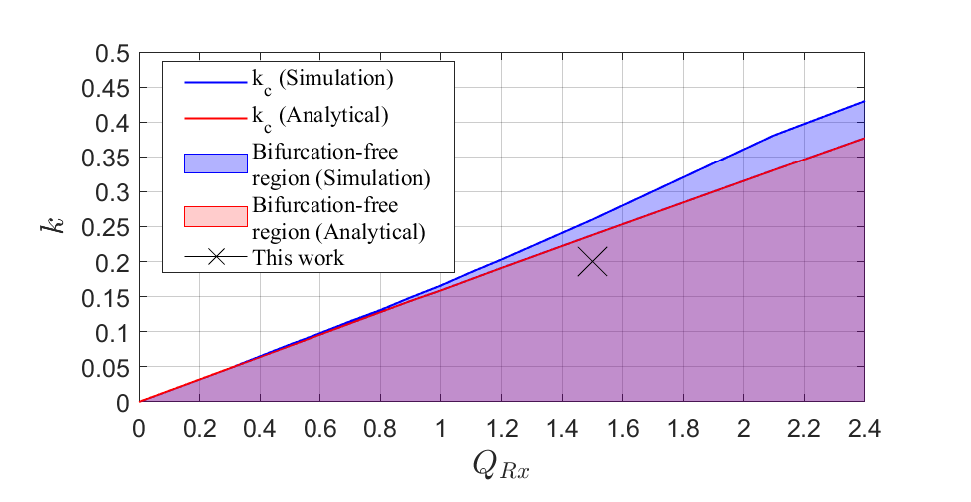
\includegraphics[width=0.92\linewidth]{critical_coupling.eps}
    \caption{Comparison of critical couplings for different $Q_{RX}$ values. }
    \label{fig:critical coupling}
\end{figure}

Firstly, the analytical design procedure is repeated along with $Q_{RX}=0.2$ to $Q_{RX}=2.2$.
For $k_{Rx,R}=0.4$ and $\Psi=1.1$,  the critical couplings are calculated by both analytical and simulation models. 
As can be seen in Fig.~\ref{fig:critical coupling}, the analytical results deviate from the simulation for higher $Q_{Rx}$~($>1$) values. 
The deviation can be ignored due to the critical coupling of the analytical model is always smaller than the simulation results. Therefore, the selected coupling below the critical value calculated by the analytical model always gives a bifurcation-free system.
Secondly, the input impedance can be expressed as in  (\ref{eq:Zin_1}) where $Z_{Rx}$, $Z_{MSR}$, $Z_{Tx}$ are provided in (\ref{eq:ZrxMSR}).

\begin{equation}
Z_{in}= Z_{Tx}+ \dfrac{\omega^2M_{Tx,MSR}^2}{Z_{MSR}+\dfrac{\omega^2M_{Rx,MSR}^2}{Z_{Rx}+R_L}}
    \label{eq:Zin_1}
\end{equation}

\begin{equation}
\label{eq:ZrxMSR}
    \begin{split}
    Z_{Rx} &= j \bigg(\dfrac{\omega^2-\omega_0^2}{\omega}\bigg) Q_{Rx} R_L \\
    Z_{MSR} &=j \bigg(\dfrac{\omega^2-\omega_0^2}{\omega} \bigg) \dfrac{V_{out^2}}{\omega_0\Psi^2I_{in}^2k_{Rx,MSR}^2Q_{Rx}R_L} \\
    Z_{Tx} &=j \bigg(\dfrac{\omega^2-\omega_0^2}{\omega}\bigg) \dfrac{\Psi I_{in}R_LV_{in^2}}{\omega_0^22I_{in}^2k_{Tx,MSR}^2Q_{MSR}Vout} \\
    \end{split}
\end{equation}


The input phase angle is zero at $\Im (Zin) =0$. The number of $\omega$ that provides this equation determines the bifurcation condition. For constant $k_{Tx,MSR}$, a lower $Q_{Rx}$  causes bifurcation, as shown in Fig. \ref{fig:critic_coupling}.a
where three zero phase angle frequencies exist.
% \hl{From a different point of view,  a higher } $k_{Tx,MSR}$ \hl {causes bifurcation. }
For constant  $Q_{Rx}$, the system is in bifurcation at a higher  $k_{Tx,MSR}$ as shown in Fig. \ref{fig:critic_coupling}.b where three zero phase angle frequencies exist.
% \hl{Therefore, a critical $k_{Tx,MSR}$ for each  $Q_{Rx}$, and critical $Q_{Rx}$ for every exist to avoid bifurcation.}
\begin{figure}[h]
    \centering
    \subfigure[$Q_{RX}$ sweeping for $k_{Tx,MSR}=0.2$.]{
    \includegraphics[width=1\linewidth]{bifurcation.png}
    }
    \subfigure[ $k_{Tx,MSR}$ sweeping for $Q_{RX}=1.5$ ]{
      \includegraphics[width=1\linewidth]{bifurcation_kc.png}
    }
    \caption{Zero phase angle frequencies ($\omega_l$, $\omega_m$, and $\omega_h$) for different $Q_{RX}$ and $k_{Tx,MSR}$.}
    \label{fig:critic_coupling}
\end{figure}


%%%%%%%%%%%%%%%%%%%%%%%%%%%
%%%%%%%%%%%%%%%%%%%%%%%%%%%%%
\subsection{The Effect of Diode Rectifier }
In this part,  the voltage gain calculated by the analytical model is compared with the simulation results.  
The analytical design methodology is based on fundamental harmonic approximation (FHA), which is presented under these assumptions: no-higher order harmonics and continuous coil current, also known as continuous current mode (CCM) \cite{3rdharmonicEnhance}.
However, an IPT system can also operate in discontinuous current mode (DCM) because of the diode rectifiers, and the low-quality factor of Rx modules \cite{3rdharmonicIET}.
In DCM, the currents of the coils have odd harmonics ($3^{rd}$, $5^{th}$), which are comparable to the fundamental component.
In our system, we observe DCM operation where the current waveforms are shown in Fig.~\ref{fig:3rd_harmonic}. 
%%%%%%%%%%%%%%%%%
\begin{figure}[h]
    \centering
    \includegraphics[width=0.9\linewidth]{third_harmonic2.png}
    \caption{1Tx-1R-1Rx current waveforms during DCM operation.}
    \label{fig:3rd_harmonic}
\end{figure}
%%%%%%%%%%%%%%%%%%%%%%
\\
Thus, the analytical model deviates due to the DCM operation, and it also causes the voltage gain to increase due to third harmonics.
The design procedure is repeated along with different $Q_{Rx}$, as shown in Fig.~\ref{fig:gain_Qrx}. 
The voltage gain is 10\% greater than the analytical calculation for our system due to DCM operation. 
However, this deviation can be tolerated since it does not affect the critical couplings.
%%%%%%%%%%%%%%%%%%%%%%%%%%%%%%%%%%%%%%
\begin{figure}[h]
    \centering
    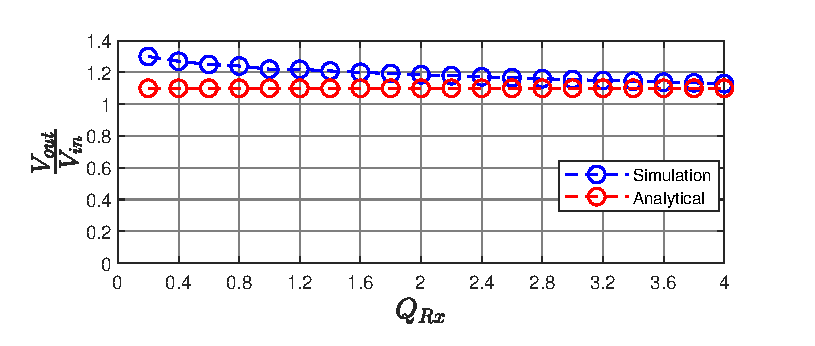
\includegraphics[width=0.9\linewidth]{gain_Qrx.eps}
    \caption{The voltage gain over different $Q_{Rx}$ for FHA based analytical model and simulation results with DCM operation.}
    \label{fig:gain_Qrx}
\end{figure}
%%%%%%%%%%%%%%%%%%%%%%%%%%%%%%
\subsection{The Effect of Cross and Direct Couplings}
The analytical model is created without consideration of the cross-couplings ( $k_{Tx,Tx}$, $k_{Rx,Rx}$) and direct couplings ($k_{Tx,Rx}$), which may change the resonant frequency, gain, and bifurcation conditions. Therefore, the analytical model should be checked with the addition of these components.

\subsubsection{The cross coupling between Tx modules}
Introducing cross-couplings between Tx modules causes an additional induced voltage component at Tx modules alongside the voltage induced by the MSR coil, which is calculated as in (\ref{eq:Mtxtx1}).

\begin{equation}
\begin{split}
    V_{in,Tx_{1}}&= \big(j\omega L_{Tx}+ \dfrac{1}{j\omega C_{Tx}}\big)I_{Tx_{1}} 
    + j\omega \big(M_{Tx_{1},Tx_{2}}\big) I_{Tx_{2}}    \\
               & + j\omega \big(M_{Tx_{1},MSR}\big)I_{MSR}    \\
            %   & + j\omega \big(M_{Tx_{1},Tx_{2}}\big) I_{Tx_{2}}   
\end{split} 
\label{eq:Mtxtx1}
\end{equation}



If these cross-couplings do not exist ($M_{Tx_{1},Tx_{2}}=0$), the resonant frequency is calculated as $f_r= \dfrac{1}{2\pi\sqrt{L_{Tx}C_{Tx}}}$.
%(\ref{eq:resonant_Tx}).
Thus, with this assumption, the resonant frequency is not affected by the Txs current, which means that the resonant frequency is equal for healthy and faulty conditions. 

However, introducing $k_{Tx,Tx}$ makes the resonant frequency sensitive to the Tx currents. The resonant frequency of one of the Tx modules is calculated as in  (\ref{eq:resonant_Tx12}).

\begin{equation}
\begin{split}
    f_r_{(Tx_{1})}= \dfrac{1}{2\pi\sqrt{ \big(L_{Tx} +\dfrac{I_{Tx2}}{I_{Tx1}}M_{Tx_{1},Tx_{2}} \big )C_{Tx}}}  
    % &f_r_{(Tx_{2})}= \dfrac{1}{2\pi\sqrt{ \bigg(L_{Tx} + \dfrac{I_{Tx1}}{I_{Tx2}}M_{Tx_{1},Tx_{2}} \bigg )C_{Tx}}}
    \end{split}
    \label{eq:resonant_Tx12}
\end{equation}

For cross-coupled Tx modules, the resonant frequency is same in healthy operation, and the Tx modules' currents are equal.
However, in faulty operation or under unbalanced Tx currents, the resonant frequency changes, which may affect the ZVS conditions, efficiency, and voltage gain. In this situation, a closed-loop frequency control can be used to adjust Tx's currents. Another solution is to minimize $k_{Tx,Tx}$ by a proper coil design, which will be discussed in section  \RomanNumeralCaps{7}. 


\subsubsection{The cross couplings between Rx modules}
The cross-couplings between the Rx modules generate additional induced voltages on each Rx module, which increase the output voltage even in healthy conditions.  
The induced voltage of one Rx module is calculated as in 
(\ref{eq:Mrxrxs}).

\begin{equation}
\begin{split}
    V_{Rx_{1}}&=j\omega M_{({Rx_{1},MSR}} I_{MSR})
               +\sum^{4}_{i=2}(j\omega M_{({Rx_{1},Rx_{2}})}I_{Rx_i})
\end{split} 
\label{eq:Mrxrxs}
\end{equation}
Moreover, the cross-couplings deviate the resonant frequency, which is calculated as in(\ref{eq:resonant_Rx1234})
% \hl{for one of the Rx module.}

\begin{equation}
    f_r_{(Rx_{1})}= \dfrac{1}{2\pi\sqrt{ 
      \Big (L_{Rx} + \sum^{4}_{i=2}  \dfrac{I_{Rx_i}}{I_{Rx_1}}M_{Rx_{1},Rx_{i}}  \Big) C_{Rx}  } }
    \label{eq:resonant_Rx1234}
\end{equation}

Another issue is the bifurcation limits. The cross-coupling changes the effective $Q_{Rx}$ as in  (\ref{eq:quality}).
\begin{equation}
  Q_{Rx}= \dfrac{\omega \big (L_{Rx}+ \sum^{4}_{i=2}M_{Rx_1,Rx_i}\big)}{R_L}
    \label{eq:quality}
\end{equation}
Therefore, positive cross-couplings increase the effective $Q_{Rx}$ and negative cross-coupling decreases the effective $Q_{Rx}$. The bifurcation limits should be updated by this variation, as previously shown in Fig. \ref{fig:critic_coupling}.


\subsubsection{The direct couplings between Tx and Rx modules}
The direct couplings between the Tx-Rx modules change the resonant frequency and voltage gain, which can be analyzed by equating the imaginary parts of the reflected impedance to Tx and the Tx side impedance, as given in  (\ref{eq:ZTx-ZMSR-ZRX}). 
\begin{equation}
  \bigg\Im\bigg(Z_{Tx}\bigg) =  -\bigg\Im\bigg(  \dfrac{\omega^2M_{Tx,MSR}^2}{Z_{MSR}}+ \dfrac{\omega^2M_{Tx,Rx}^2}{Z_{Rx}}   \bigg)
    \label{eq:ZTx-ZMSR-ZRX}
\end{equation}
The input and output voltage formulas are modified as given in  (\ref{eq:Vin-Vout}). 
The $M_{Tx,MSR}$ and $M_{Rx,MSR}$ should be adjusted if the voltages are desired to be the same as the voltages without direct-couplings. 
\begin{equation}
\begin{split}
    V_{in} &= \omega_{0}I_{MSR}M_{Tx,MSR}\angle{\phi_{I_{MSR}}}+\omega_{0}I_{Rx}M_{Tx,Rx}\angle{\phi_{I_{Rx}}} \\
    V_{out} &= \omega_{0}I_{MSR}M_{Rx,MSR}\angle{\phi_{I_{MSR}}}+ \omega_{0}I_{Tx}M_{Tx,Rx} 
\end{split}
    \label{eq:Vin-Vout}
\end{equation}

\subsection{The Effect of Mechanical Rotation}
A circular MSR coil creates a rotational symmetry, which provides constant $M_{Tx,MSR}$ and $M_{Rx,MSR}$. However, if an axial misalignment occurs (due to the manufacturing tolerances) between stationary and rotating parts.
$M_{Tx,MSR}$ becomes a function of rotation angle. In an analytical model, the induced voltage onto MSR coil from Tx coils depends on $M_{Tx,MSR}$, $I_{Tx}$, $\omega$ as shown in (\ref{eq:VMSR}). 
\begin{equation}
    \label{eq:VMSR}
    \begin{split}
         V_{MSR}_{(t)} &= \dfrac{d}{dt} M_{Tx,MSR} \hat{I}_{Tx}sin(\omega t+ \phi_{I_{Tx}}) 
        %  V_{MSR} &= j \omega M_{Tx,MSR} I_{Tx}
    \end{split}
\end{equation}
However, a variable $M_{Tx,MSR}$ induces extra components, as given  (\ref{eq:VMSR2}) where $\omega_m$ is the mechanical angular frequency. In order to simplify the calculation, $M_{Tx,MSR}$ is assumed to be a sine function  with the peak value of $\hat{M}_{Tx,MSR}$.
\begin{equation}
    \label{eq:VMSR2}
    \begin{split}
         V_{MSR}_{(t)} &= \dfrac{d}{dt} \hat{M}_{Tx,MSR} \hat{I}_{Tx}sin(\omega t+ \phi_{I_{Tx}}) \\ &+ \dfrac{d}{dt} \hat{M}_{Tx,MSR}sin(\omega_m t)\hat{I}_{Tx} 
        %  V_{MSR} &= j \omega \hat{M}_{Tx,MSR} \hat{I}_{Tx} + j \omega_m \hat{M}_{Tx,MSR} \hat{I}_{Tx}
    \end{split}
\end{equation}
Furthermore, the operating frequency of IPT  is about 150 kHz, and the rated rotational speed of the system is 1500 RPM, which is equal to 25 Hz. Since there are 6000 periods in one full rotation, the IPT system can be assumed to be stationary.
The induced voltage coming from the change in mutual is less than 0.02\% of the induced voltage from the Tx current. Therefore, the effect of the mechanical rotation can be ignored.


\section{The Proposed Coil Geometry }
This section presents the proposed coil geometry to minimize cross-couplings and direct couplings. As previously shown in Fig. \ref{fig:rotational_coil}, the Tx and Rx coils are designed to create a full circle, delivering magnetic symmetry for the rotation.
\begin{figure}[h]
    \centering
    \includegraphics[width=1\linewidth]{CoilStructure3.png}
    \caption{The proposed coil structure to minimize cross-couplings as shown from the side-view.}
    \label{fig:coil_structure}
\end{figure}

The coils should provide the self and mutual inductances while keeping the cross-coupling and direct couplings at minimum to avoid resonant frequency and gain deviations.
Firstly, Tx coils are formed as half-circles as shown in Fig. \ref{fig:rotational_coil}, but in this configuration, end-windings cause cross-couplings. 
Then, the coils are modified by bending the end-windings, and placing ferrite, as shown in Fig. \ref{fig:coil_structure}.
Thus, the magnetic field is shielded, and the cross-couplings can be minimized. 
A finite element analysis is made to observe the effect of the bending of the end-windings. The results are given for the straight and bent Tx coil end-windings in  (\ref{equ:inductancematrix}). 
It is shown that bending of Tx coil end-windings helps to reduce the cross-coupling by half.

\begin{equation}
    \label{equ:inductancematrix}
    L_{Tx1,Tx2}(\mu H)= 
    \begin{cases}
        \begin{bmatrix}
        80.5 & -6.3\\
        -6.3 & 80.5 \\
        \end{bmatrix}  & \text{Straight Txs}  \\
        \\
        \begin{bmatrix}
        80.8 & -3.3 \\
        -3.3 & 80.8 \\
        \end{bmatrix}  & \text{Bent Txs}
    \end{cases}
\end{equation} 


Secondly, the MSR coil can be designed as two coils connected in series, the one is coupled with Tx coils, and the second is coupled with the Rx coils. The coils are magnetically isolated by the ferrite strips between them, as shown in Fig.  \ref{fig:coil_structure}.
Finally, the cross-couplings between Rx modules can be minimized by bending the end windings like the Tx modules. 
Alternatively, high frequency coupled inductors (HFCI) can be used to couple the MSR and Rxs coils.
Unlike most IPT systems,  air gap of the proposed system can be adjusted.
Furthermore, the couplings between the MSR and Rxs can be increased to reduce the resonator coil size, which is not limited by the bifurcation phenomena.
Since the direct couplings between Tx and Rx coils should be minimized,  the MSR coil can be separated into five coils that are connected in series, where one coil couples with Tx coils and the other four coils couple with Rx coils using HFCIs. 
Using HFCIs provides tightly-coupled coils, which is not achieved by the conventional circle and quarter-circle coils.   
The proposed coil configuration is shown in Fig. \ref{fig:HFCI_anlatim}.
Here, $L_{MSR}$ is the sum of $L_{MSR(Tx)}$, $L_{MSR(Rx1)}$, $L_{MSR(Rx2)}$, $L_{MSR(Rx3)}$, and $L_{MSR(Rx4)}$. While  $L_{MSR(Tx)}$ is achieved via a conventional circular coil, the other inductances are achieved via HFCIs.

\begin{figure}[h!]
    \centering
    \includegraphics[width=1\linewidth]{HFCI_anlatim.pdf}
    \caption{The proposed coil configuration of the proposed system using HFCIs.}
    \label{fig:HFCI_anlatim}
\end{figure}

\begin{figure}[h!]
    \centering
    \includegraphics[width=1\linewidth]{opposite_direction.png}
    \caption{The eddy currents induced on the mechanical shaft for a single Tx-Rx system. (a) Same current direction for inner and outer coils. b) Opposite current direction for inner and outer coils. }
    \label{fig:opposite}
\end{figure}

Furthermore, the proposed coil geometries minimize the eddy losses of the motor's conducting (mechanical) shaft. The proposed Tx coils have inner and outer windings carrying currents in opposite directions. 
Therefore, the eddy currents on the shaft can be decreased compared to conventional circular coils, as shown in Fig. \ref{fig:opposite}. 
In addition, for Rx modules, HFCI cores guide the magnetic flux, so the magnetic flux outside the HFCI is almost zero. The frame of motors is also electrically conducting, so  eddy currents can be induced due to the leakage flux.
Therefore, ferrite strips, which guide the magnetic fluxes in the desired direction, can be included to reduce eddy currents.

\begin{figure}[h!]
\centering
\includegraphics[width=1\linewidth]{experimental_setup2.png}
% \includegraphics[width=1\linewidth]{Figures/experimental/experiment_setup.png}
% \caption{Experimental setup for the proposed IPT system \cite{polat_2021}}
\caption{ Experimental setup. a) Overall System. b) The proposed IPT system.}
\label{fig:experimentalsetup}
\end{figure}

%%%%%%%%%%%%%%%%%%%%%%%%%%%%%%%%%%

\section{Experimental Results }
To verify the proposed system, a 1~kW 2Tx/1MSR/4Rx prototype is built as shown in Fig.~\ref{fig:experimentalsetup}. The parameters of the experimental setup are shown in Table~\ref{tab:experimetalsetupparameters}. In order to achieve high fault tolerance, Rx modules are over-designed, which provides the system to transfer rated power under Rx faults. 
HFCIs are designed with ferrites (PQ32x20 with N87 material) with an air gap of 0.4~mm. The parameters of which are presented in Table~\ref{tab:experimetalsetupparameters}. 
As shown in the table, $M_{Rx,MSR}$ inductances are practically identical, and there is no cross-coupling between them as expected.  
%%%%%%%%%%%%%%%%%%%%%%%%%%%%%%%%
%%%%%%%%%%%%%%%%%%%%%%%%%%%%%%%%
%%%%%%%%%%%%%%%%%%%%%%%%%
\begin{table}[h]
\centering
\caption{Experimental Setup Parameters}
\label{tab:experimetalsetupparameters}
\begin{tabular}{ll}
\hline \\
Tx side MOSFET       &   BSC600N25NS3G   \\
Tx side Gate Driver       &  2EDF7275F     \\
Rx side Recrifier Diodes       &  C3D10060G      \\
Litz Wire     & 400x0.08~mm ($\mathrm{2~mm^2}$)      \\
Ferrite shield   &   I20x2 N48     \\
Tx coil $\mathrm{D_{in}}$ and $\mathrm{D_{out}}$  &  70-280 mm\\
Tx coil \# of turns         &   13      \\
Tx coil inductances        &  83.1-83.5 $\mathrm{\mu H}$\\
Mutual inductance between Tx coils    &  3.5 $\mathrm{\mu H}$\\
Resonator IPT coil $\mathrm{D_{in}}$ and $\mathrm{D_{out}}$ &  65-280 mm\\
Resonator IPT coil \# of turns         &   5      \\
Resonator IPT coil inductance  & 23 $\mathrm{\mu H}$\\
$\mathrm{C_{Tx}}$         &   13.6 ~nF    \\
$\mathrm{C_{R}}$         &   15.21 ~nF   \\
$\mathrm{C_{Rx}}$        &   44.2 ~nF   \\
Airgap   &   10 (mm)     \\
Resonant frequency ($\mathrm{f_0}$)  &   150~kHz      \\
Operating frequency ($\mathrm{f}$)  &   155~kHz      \\
\hline
\end{tabular}

\begin{tabular}{lllll}
\\
\multicolumn{5}{c}{\textbf{Parameters of the High Frequency Coupled Inductors}} 
\\
\hline
\hline
Parameters & \textbf{$\mathrm{HFCI_{1}}$} &\textbf{$\mathrm{HFCI_{2}}$}& \textbf{$\mathrm{HFCI_{3}}$}& \textbf{$\mathrm{HFCI_{4}}$}\\ \hline
\textbf{$L_{MSR}(\mu H)$} & 13.37& 13.27  &  13.19&13.25 \\
\textbf{$L_{Rx}(\mu H)$}& 26.88&  26.85 &  26.89 &  27.07        \\
\textbf{$M(\mu H)$} & 18.05  & 18.14&  18.01 & 18.09   \\
\hline
\multicolumn{3}{c}{Core Size} & \multicolumn{2}{c}{PQ 35x35} \\
\multicolumn{3}{c}{Core Material} & \multicolumn{2}{c}{N87} \\
\multicolumn{3}{c}{Airgap} & \multicolumn{2}{c}{0.4~mm} \\
\multicolumn{3}{c}{Number of R Turns} & \multicolumn{2}{c}{6} \\
\multicolumn{3}{c}{Number of Rx Turns} & \multicolumn{2}{c}{9} \\
\hline
\end{tabular}

\end{table}
%%%%%%%%%%%%%%%%%%%%%%%%%%%%%%%%%

%%%%%%%%%%%%%%%%%%%%%%%%%%%%%%%%
The MSR coil is wound as circle-shaped, and two Tx coils are wound as half-circle-shaped, merging into a full circle. 
The Tx coils are isolated from each other by bent end-winding configuration and with extra ferrite strips. 
However, Tx coils still have slight cross-coupling, and  mutual inductance between them is measured as $3.5 \mu H$. 
Also, mutual inductances between the MSR and Tx coils vary with rotation due to small axial misalignments and manufacturing tolerances. 

The fluctuation is measured experimentally for both Tx coils, and presented in Fig. \ref{fig:mutual_change}. The maximum fluctuation is below 12\%, and practically no significant voltage term is inducted as discussed in. (\ref{eq:VMSR2}).

\begin{figure}[h!]
   \centering
\includegraphics[width=0.90\linewidth]{Mutual_change_v2.eps}
     \caption{The percentage of the $M_{Tx,MSRr}$ fluctuation over a full mechanical rotation.}
        \label{fig:mutual_change}
\end{figure}
%%%%%%%%%%%%%%%%%


%%%%%%%%%%%%%%%%%%%%%%%%%%%%%%%%%%%%%%%
\subsection{System Tests}
Several operating conditions are tested with the given experimental setup. The healthy operation of the system is verified at first. Then faulty conditions are tested. Detailed results are discussed in the following sections.
%%%%%%%%%%%%%%%%%%%%%%%%%%%%%%%%%%%%%%%%
\subsubsection{Normal Operation}
%%%%%
%%%%%%
Firstly, the system is operated at 156~kHz, slightly above the resonant frequency, which satisfies the zero voltage switching. 
The experimental results under normal operation are given in Fig.~\ref{fig:normaloperation}. 
The Rx currents are nearly equal and have a third harmonic component. 
The reflected third harmonic component can also be seen at the resonator current.
Resonator currents are slightly smaller than the Tx current in experimental results due to the losses, which are not included in the analytical model.
\begin{figure}[h!]
   \centering
        	\includegraphics[width=0.90\linewidth]{healthy_new3.png}
     \caption{Input voltage, Tx side currents, resonator current and Rx currents for healthy operation. ($I_{Tx1,2}\approx 6.5~A_{rms},I_{R}=5.4~A_{rms}$)  }
        \label{fig:normaloperation}
\end{figure}
%%%%%%%%%%%%%%%%%%%%%%%%%%%%%%%%%%

\subsubsection{Single and Double Rx Open Circuit Fault}
%%%%%
In Fig.~\ref{fig:results}.a, operation under a single Rx open circuit fault is presented. Results are similar to healthy operation, and the third harmonic component is reduced compared to the healthy operation. 
Since Rxs are over-designed in the experimental setup, the rated power is transferred; otherwise, the transferred power should be reduced as presented in (\ref{eq:P_Rxfault}). 
Increasing the number of Rx modules will result in less stress on the remaining modules under fault; however, it also increases the chance of a failure due to the increased number of components.
Then the effect of simultaneous faults in two Rx modules is investigated. 
The results are presented in Fig.~\ref{fig:results}.b. 
The effective quality factor of the Rx modules becomes greater than healthy operation since the current of the remaining modules increases. Hence, the system operates in CCM, and the third harmonic is almost diminished. 
%%%%%%%%%%%%%%%%%%%%%%%%%%%%%%%%%%%
\subsubsection{Single Tx Open Circuit Fault}
Finally, the fault tolerance of the system is tested with a single open circuit Tx fault. 
As the Tx modules are not over-designed, the power is reduced from 1000W to 250W, as shown in Fig.~\ref{fig:results}.c.
Under an open-circuited Tx fault, the flux linkage is reduced by half, which also decreases the resonator current, but the power is shared between the Rx modules equally.
The rated power could be transferred if Tx modules are over-designed.

 \begin{figure*}[]
     \centering
        	\includegraphics[width=1\linewidth]{faulty_new3.png}
        \caption{The waveforms of input voltage, Tx side currents, resonator current and Rx currents for faulty operations. a) Single open circuited Rx fault. b) Double open circuited Rx fault. c) Single open circuited Tx fault. }
        \label{fig:results}
\end{figure*}
%%%%%%%%%%%%%%%%%%%%

\begin{table}[h!]
\centering
\caption{Efficiencies of the System Under Healthy and Faulty Operations }
\label{tab:efficiency}
\begin{tabular}{lc}
\centering
\textbf{Operation} & Efficiency\\
\hline
\textbf{Healthy operation} &  90.9 \% \\
\textbf{Single Rx open faulty operation} &  89.6 \% \\
\textbf{Double Rx open faulty operation}  & 89.5   \%  \\
\textbf{Single Tx faulty operation}&  81.6  \%  \\
\hline
\end{tabular}
\end{table}
%%%%%%%%%%%%%%%%%%%%%%

%%%%%%%%%%%%%%%%
\subsubsection{Efficiency under fault}
The system efficiencies under healthy and faulty operations are given in Table~ \ref{tab:efficiency}.
Single-Tx fault's efficiency is lower than healthy operation due to lower input voltage as expected.
However, Txs have the same voltage and current value in single-Rx and double-Rx faults, providing compatible efficiency with the healthy operation, which confirms the fault tolerance of the proposed system. 
%%%%%%%%%%%%%%%%%%%%%%

\section{Comparison with Existing Studies in the Literature}
A few contactless energy transfer systems in the literature are presented in the Table. \ref{tab:comparison_literature}.  Inductive power transfer (IPT) and capacitive power transfer (CPT) systems are commonly used, depending on the airgap and power requirements.

\begin{table}[h]
\centering
\caption{ Comparison with existing studies in the literature}

\begin{tabular}{l|c|c|c|c|c}
         & \textbf{\cite{table-2}} & \textbf{\cite{table-3}}   & \textbf{\cite{table-8}}       & \textbf{\cite{table-10}}      &  \textbf{\begin{tabular}[c]{@{}l@{}}This \\ work \end{tabular}} \\ \hline \hline
\textbf{ \begin{tabular}{ll}  Coil   \\ Type \end{tabular} }  
& \begin{tabular}{ll}  1Tx \\ 1Rx \end{tabular}  
& \begin{tabular}{ll}  1Tx \\ 1Rx \end{tabular}   
& \begin{tabular}{ll}  1Tx \\ 1Rx \end{tabular}   
& \begin{tabular}{ll}  1Tx \\ 1Rx \end{tabular}  
&  \begin{tabular}{ll} 2Tx \\ 1MSR \\4Rx  \end{tabular}      
   \\ \hline         

\textbf{ \begin{tabular}{ll}
     Topology \\ 
\end{tabular} }   & CPT        & IPT           & IPT         & IPT     &     IPT               \\ \hline

         
\textbf{ \begin{tabular}{ll}
     Frequency \\ (kHz)
\end{tabular} }          & $>$650    & 250      & 50        & 50    &   150                  \\ \hline


\textbf{ \begin{tabular}{ll}
     Power \\ (W)
\end{tabular} }  & 340        & 300       & 500        & 1000    & 1000            \\ \hline

\textbf{ \begin{tabular}{ll}
     Airgap \\ (mm)
\end{tabular} }   & 0.081      & 18             & -         & 0.6                      &   10                 \\ \hline


\textbf{ \begin{tabular}{ll}
     Diameter \\ (mm)
\end{tabular} }  & 76.2       & 120               & 100         & -      &    280                \\ \hline

\textbf{ \begin{tabular}{ll}
     Efficiency \\ (\%)
\end{tabular} } & 85         & 92-95  & \textgreater{}80 &     92.7   &  90.9        \\ \hline \hline


\end{tabular}
\label{tab:comparison_literature}
\end{table}



\begin{table}[h!]
\centering
\caption{The performance comparison of the proposed system}
\begin{tabular}{|c|ccc|c|}
\hline
\multirow{2}{*}{\textbf{\begin{tabular}[c]{@{}c@{}}Performance \\ Metrics\end{tabular}}} & \multicolumn{3}{c|}{\textbf{Retrieved from \cite{table-2}}}                    & \multirow{2}{*}{\textbf{\begin{tabular}[c]{@{}c@{}}This \\ Study\end{tabular}}} \\ \cline{2-4}
   & \multicolumn{1}{c|}{\textbf{\begin{tabular}[c]{@{}c@{}}Slip \\ Rings\end{tabular}}} & \multicolumn{1}{c|}{\textbf{\begin{tabular}[c]{@{}c@{}}Inductive\\ Couplers\end{tabular}}} & \textbf{\begin{tabular}[c]{@{}c@{}}Capacitive \\ Coupler\end{tabular}} &                                                                                         \\ \hline
\textbf{\begin{tabular}[c]{@{}c@{}}Maintenance \\ Requirement\end{tabular}}       & \multicolumn{1}{c|}{Yes}                                                        & \multicolumn{1}{c|}{No}                                                         & No                                                                       
& \textcolor{black}{No}                                                                    
         
         \\ \hline

\textbf{\begin{tabular}[c]{@{}c@{}}Fault \\ Tolerance\end{tabular}}               & \multicolumn{1}{c|}{No}                                                          & \multicolumn{1}{c|}{No}               
& \multicolumn{1}{c|}{No}      
& \multicolumn{1}{c|}{ \textcolor{black}{Yes}}                       

\\ \hline

\textbf{\begin{tabular}[c]{@{}c@{}}Speed\\ Sensitivity\end{tabular}}              & \multicolumn{1}{c|}{Yes}                                               
& \multicolumn{1}{c|}{No}                                                         & Possible                                                               
& \textcolor{black}{No}                                                                                      \\ \hline

\textbf{Scalability}                                                               & \multicolumn{1}{c|}{Diffucult}                                                   
& \multicolumn{1}{c|}{Possible}                                                    & Possible                                                               
& \textcolor{black}{Easy}                                                                                      \\ \hline

\textbf{\begin{tabular}[c]{@{}c@{}}Output\\ Side\end{tabular}}                   & \multicolumn{1}{c|}{DC}                                                          & \multicolumn{1}{c|}{\begin{tabular}[c]{@{}c@{}}Single\\ Rectifier\end{tabular}} & \multicolumn{1}{c|}{\begin{tabular}[c]{@{}c@{}}Single\\ Rectifier\end{tabular}} & \multicolumn{1}{c|}{\begin{tabular}[c]{@{}c@{}} \textcolor{black}{Multiple}\\ \textcolor{black}{Rectifiers}\end{tabular}}                                                                                   
\\ \hline

\textbf{\begin{tabular}[c]{@{}c@{}}Input \\ Side\end{tabular}}                         & \multicolumn{1}{c|}{\begin{tabular}[c]{@{}c@{}} DC\end{tabular}}         
& \multicolumn{1}{c|}{\begin{tabular}[c]{@{}c@{}}Single\\ Converter\end{tabular}} & \begin{tabular}[c]{@{}c@{}}Single \\ Converter \end{tabular}                 
& \begin{tabular}[c]{@{}c@{}} \textcolor{black}{Multiple} \\ \textcolor{black}{Converters} \end{tabular}                                  
\\ \hline

\textbf{Size}                                                                      & \multicolumn{1}{c|}{Small}                                                       & \multicolumn{1}{c|}{Medium}                                                      & Medium                                                                
% &  \textcolor{cyan}{Medium}       
& \begin{tabular}[c]{@{}c@{}} \textcolor{black}{Medium-} \\ \textcolor{black}{Large} \end{tabular}    
\\ \hline

% \textbf{Cost}                                                                      & \multicolumn{1}{c|}{Low-priced}                                                  & \multicolumn{1}{c|}{Mid-priced}                                                  & Mid-priced                                                                
% & \textcolor{red}{High-priced }                                                                                 \\ \hline

\end{tabular}
\label{tab:performance_metrics}
\scriptsize
% \begin{flushleft}
%   \item  \textcolor{green}{Green: Advantages}, \textcolor{cyan}{Cyan: Neutral},  \textcolor{red}{Red: Disadvantages}
%  \end{flushleft}
\end{table}

In this article, unlike the conventional systems, a modular structure is presented, providing a reliable system that can even operate under fault. 
The performance comparison of the proposed system with other alternatives is presented in Table \ref{tab:performance_metrics}. Inductive and capacitive couplers are advantageous to slip rings in terms of maintenance. However, they are still prone to faults, and their fault tolerance can be increased by adding redundant converters. 
However, redundant converters increase the cost and complexity of the system.
Besides, adding redundant converters for a 1Tx/1Rx system requires to use of the same power ratings for all redundant converters. 
In this study, a multi-Tx/multi-Rx system is used to share the power.
Therefore, the power ratings of the converters can be decreased, reducing the cost compared to adding identical redundant converters while still increasing the fault tolerance and reliability.
However,  in the proposed multi-Tx/ multi-Rx system, an MSR coil is used to share power equally between the modules. 
It seems to create a new single point of failure like the 1Tx-1Rx system, but the failure expectation for MSR, which comprises only passive components such as inductors and capacitors (film or multi-layer ceramic capacitors), is much lower than active semiconductor devices. 
Unequal power distribution between Rx modules can exist due to minor coupling differences without the MSR coil. In this situation, the modules can exceed their power ratings, which reveals a reliability issue.
Moreover, the modular structure allows the system to operate under the failure of more than one module. 
Even though they cannot transfer rated power, under multiple faulty modules, the healthy modules can still transfer their nominal power.
Furthermore, the system's power can be upscaled or downscaled by adding or taking out the modules, so the system has good scalability, which is significant for adapting the proposed system into conventional systems.
However, using too many modules should be avoided as it may reduce the effective space of the coils. 


\section{Conclusion}
%%%%%%%%%%%%%%%%%%%%%%%%
This paper proposes a multi-Tx/multi-Rx system as an alternative to conventional slip rings for field excited synchronous machines. 
Thus, fault-tolerant and maintenance-free contactless energy transfer systems are achieved. 
However, multi-Tx/multi-Rx systems are prone to unequal power-sharing between modules, reducing reliability. 
Therefore, a novel solution, introducing a middle-stage resonator, is presented to improve unequal power-sharing. 
Furthermore, the efficiency competing with the conventional slip rings is achieved by avoiding bifurcation, which guarantees zero voltage switching.
In this paper, firstly, the design methodology of a multi-Tx/multi-Rx IPT system with a middle-stage resonator was presented. 
Then,  a fault tolerance analysis was examined, and the selection of modules number was discussed. 
Finally,  a 1 kW 2Tx/1MSR/4Rx prototype was built to validate the proposed system, and it was observed that the experimental results are coherent with analytical results under single-Rx, double-Rx, and single-Tx faults.
Consequently, a fault-tolerant multi-Tx/ multi-Rx IPT system to excite the field of synchronous machines is achieved, decreasing maintenance requirements and increasing reliability.  

%%%%%%%%%%%%%%%%%%%%%%%%%%%%%
\bibliographystyle{IEEEtran}
\bibliography{ref.bib}
% \vspace*{-20mm}
\begin{IEEEbiography}[{\includegraphics[width=1\linewidth]{enes1.jpg}}]
{Enes Ayaz} received the B.Sc. degree from the Department of Electrical and Electronics Engineering, Middle East Technical University (METU), Ankara, Turkey, in 2019, where he is currently pursuing the M.Sc. degree.

His current research interests include resonant converters, wireless power transfer, and power electronics.
\end{IEEEbiography}
% \vspace*{-130mm}
\begin{IEEEbiography}[{\includegraphics[width=1\linewidth ]{ogunaltun1.png}}]
{Ogün Altun} received his B.Sc degree from the Department of Electrical and Electronics Engineering, Middle East Technical University, Ankara, Turkey in 2020. He is pursuing his M.Sc. degree at Middle East Technical University. 

His current research interests are power converters, renewable energy, and wireless power transfer.
\end{IEEEbiography}

\begin{IEEEbiography}[{\includegraphics[width=1\linewidth ]{hakan.PNG}}]
{Hakan Polat} received the B.Sc. and M.Sc. degrees from the Department of Electrical and Electronics Engineering, Middle East Technical University (METU), Ankara, Turkey, in 2018 and 2021.Then, he joined Vrije Universiteit Brussels- MOBI EPowers as a Ph.D. student in 2021 and is currently pursuing a Ph.D. His current research interests include electric car chargers, renewable energy, resonant converters, and wireless power transfer.
\end{IEEEbiography}

% \vspace*{-130mm}
\begin{IEEEbiography}[{\includegraphics[width=1\linewidth ]{ozan.png}}]
{Ozan Keysan} received the master’s degree from Middle East Technical University (METU), Ankara, Turkey, in 2008, and the Ph.D. degree from The University of Edinburgh, Edinburgh, U.K., in 2014. 
He is currently an Associate  Professor with the Department of Electrical and Electronics Engineering, METU. 
His current research interests include wireless power transfer, renewable energy, design and optimization of electrical machines, smart grids, superconducting machines, and permanent-magnet machines.
\end{IEEEbiography}

% \vfill
\end{document}
